\documentclass[tikz, margin=5mm]{standalone}
\usetikzlibrary{arrows}
\usepackage{amsmath}
\usepackage{mathtools} 
\begin{document}
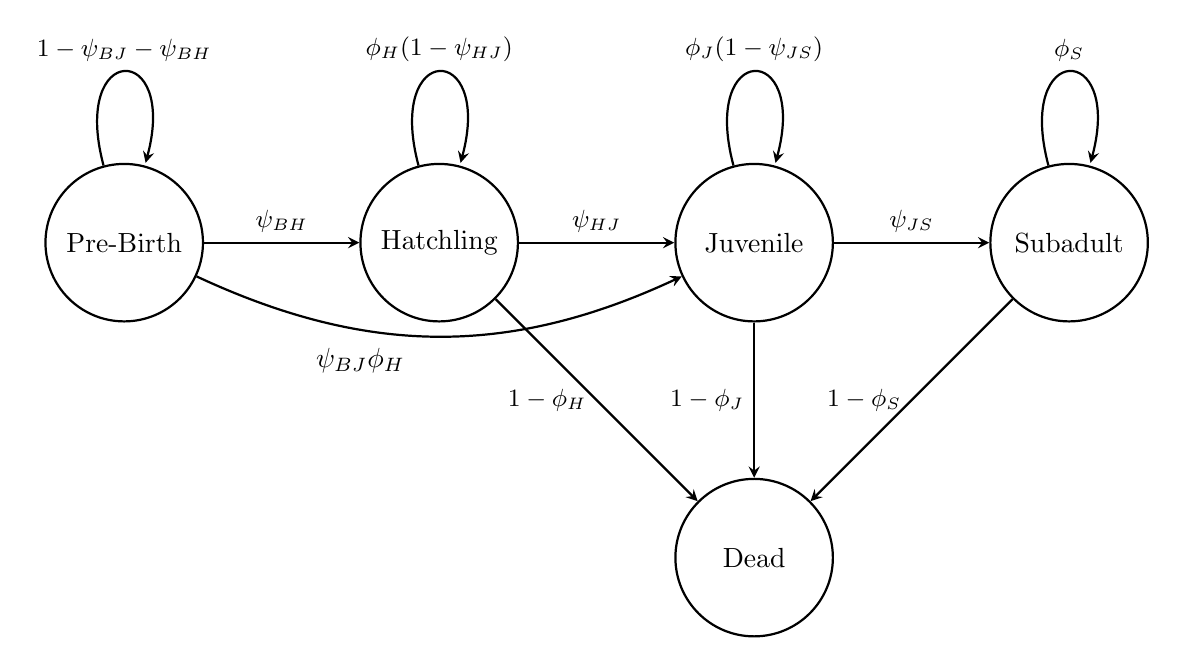
\begin{tikzpicture}
  [
    ->,
    >=stealth,
    auto,node distance=4cm,
    thick,
    main node/.style={circle, draw, minimum size = 2 cm}
    ]
   \tikzstyle{arrow} = [thick,->,>=stealth]

  \node[main node] (1) {Pre-Birth};
  \node[main node] (2) [right of = 1]  {Hatchling};
  \node[main node] (3) [right of=2] {Juvenile};
  \node[main node] (4) [right of=3] {Subadult};
  \node[main node] (5) [below of = 3] {Dead};

  \path[every node/.style={font=\sffamily\small}]
    (1) edge node [above] {$\psi_{BH} $} (2)
    (2) edge node [above] {$\psi_{HJ}$} (3)
    (3) edge node [above] {$\psi_{JS}$} (4);
  \path[->, every node/.style={font=\sffamily\small}]
  (2) edge [loop above] node {$\phi_H(1-\psi_{HJ})$} ()
  (3) edge [loop above] node {$\phi_J(1-\psi_{JS})$} ()
  (4) edge [loop above] node {$\phi_S$} ()
  (1) edge [loop above] node {$1- \psi_{BJ} - \psi_{BH}$} ()
  (2) edge node [left] {$1 - \phi_H$} (5)
  (3) edge node [left] {$1- \phi_J$} (5)
  (4) edge node [left] {$1- \phi_S$} (5)
  (1) edge [out = -25, in = -155] (3);
  
  \coordinate (point) at (3,-1.5);
  \node at (point) {$\psi_{BJ} \phi_H $};
  
  

\end{tikzpicture}
\end{document}